\documentclass[UTF8]{ctexart}
\usepackage[left=2cm,right=2cm,top=2cm]{geometry}
\usepackage{amsmath}
\usepackage{enumitem}
\usepackage{float}
\usepackage{threeparttable}
\usepackage{caption}
\usepackage{multirow}
\usepackage{graphicx}
\usepackage{listings}
\usepackage{color}
\definecolor{dkgreen}{rgb}{0,0.6,0}
\definecolor{gray}{rgb}{0.5,0.5,0.5}
\definecolor{mauve}{rgb}{0.58,0,0.82}
\lstset{frame=tb,
  language=C++,
  aboveskip=3mm,
  belowskip=3mm,
  showstringspaces=false,
  columns=flexible,
  basicstyle={\small\ttfamily},
  numbers=left,%设置行号位置none不显示行号
  %numberstyle=\tiny\courier, %设置行号大小
  numberstyle=\tiny\color{gray},
  keywordstyle=\color{blue},
  commentstyle=\color{dkgreen},
  stringstyle=\color{mauve},
  breaklines=true,
  breakatwhitespace=true,
  escapeinside=`,%逃逸字符(1左面的键),用于显示中文例如在代码中`中文...`
  tabsize=4,
  extendedchars=false %解决代码跨页时,章节标题,页眉等汉字不显示的问题
}

\setlength\lineskiplimit{5.25bp}
\setlength\lineskip{5.25bp}

\title{计算方法第五次编程作业报告}
\author{崔士强 PB22151743}
\date{\today}

\bibliographystyle{plain}

\begin{document}

\maketitle

\section{问题描述}
实现三次样条插值算法。给定若干插值点,利用大M法计算三次样条插值函数,以模拟通过弹性木条在集中载荷下自然形成的曲线。

\section{问题分析}
先从文件中读取各个点的信息,按照大M值之间的关系构造线性方程组。该方程组的系数矩阵是三对角矩阵,因此可以用追赶法求解。解出$M$值后便可得到
各个区间的三次函数表达式。

\section{实验结果}
\subsection{结果展示}
程序的计算结果如下图所示(系数按幂降序排列)
\begin{figure}[H]
  \centering
  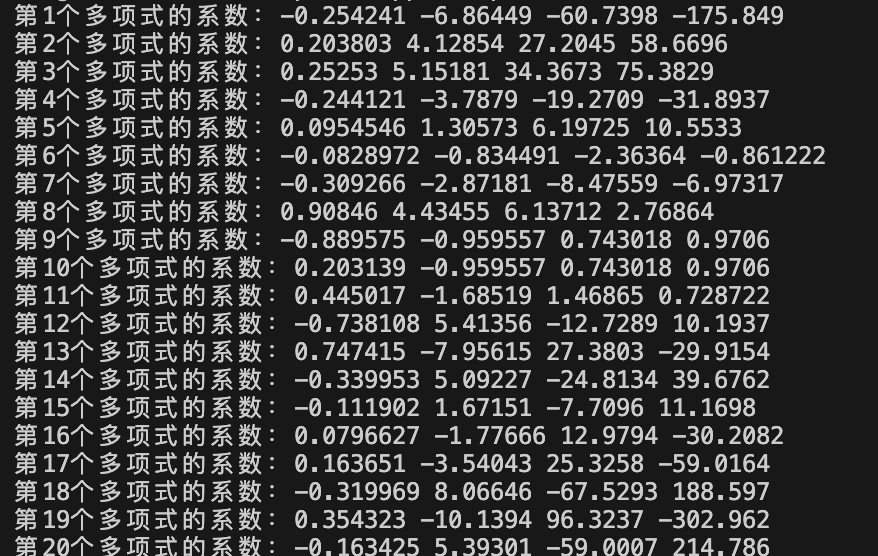
\includegraphics[scale=0.5]{res1.png}
  \caption{计算结果}
\end{figure}
\begin{figure}[H]
  \centering
  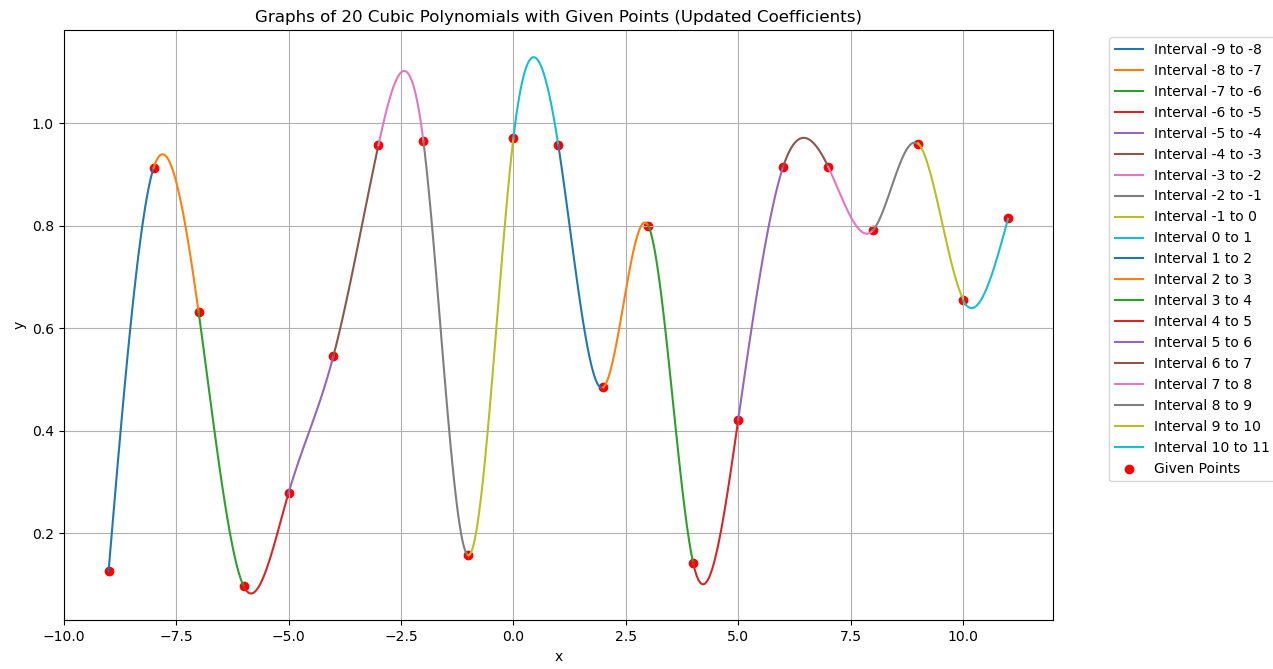
\includegraphics[scale=0.3]{Figure_1.png}
  \caption{结果可视化}
\end{figure}
\begin{figure}[H]
  \centering
  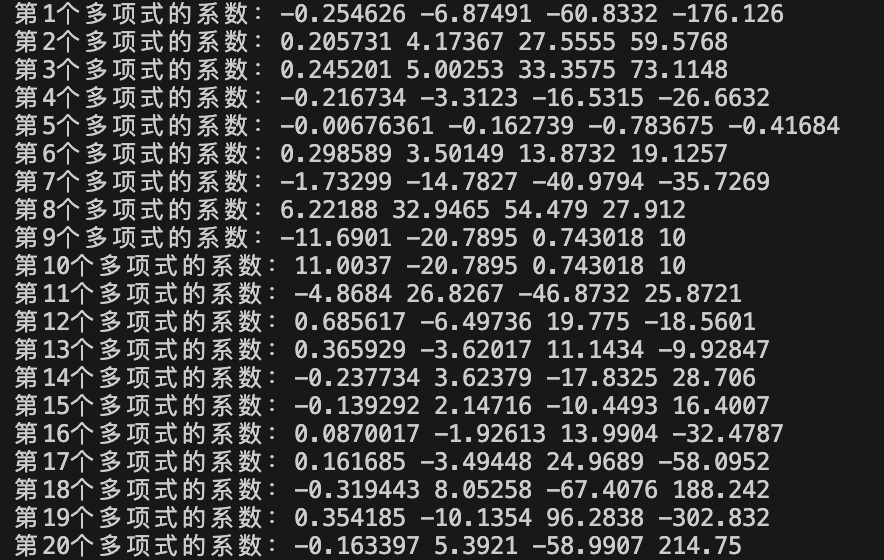
\includegraphics[scale=0.5]{res2.png}
  \caption{更改后的计算结果}
\end{figure}
\begin{figure}[H]
  \centering
  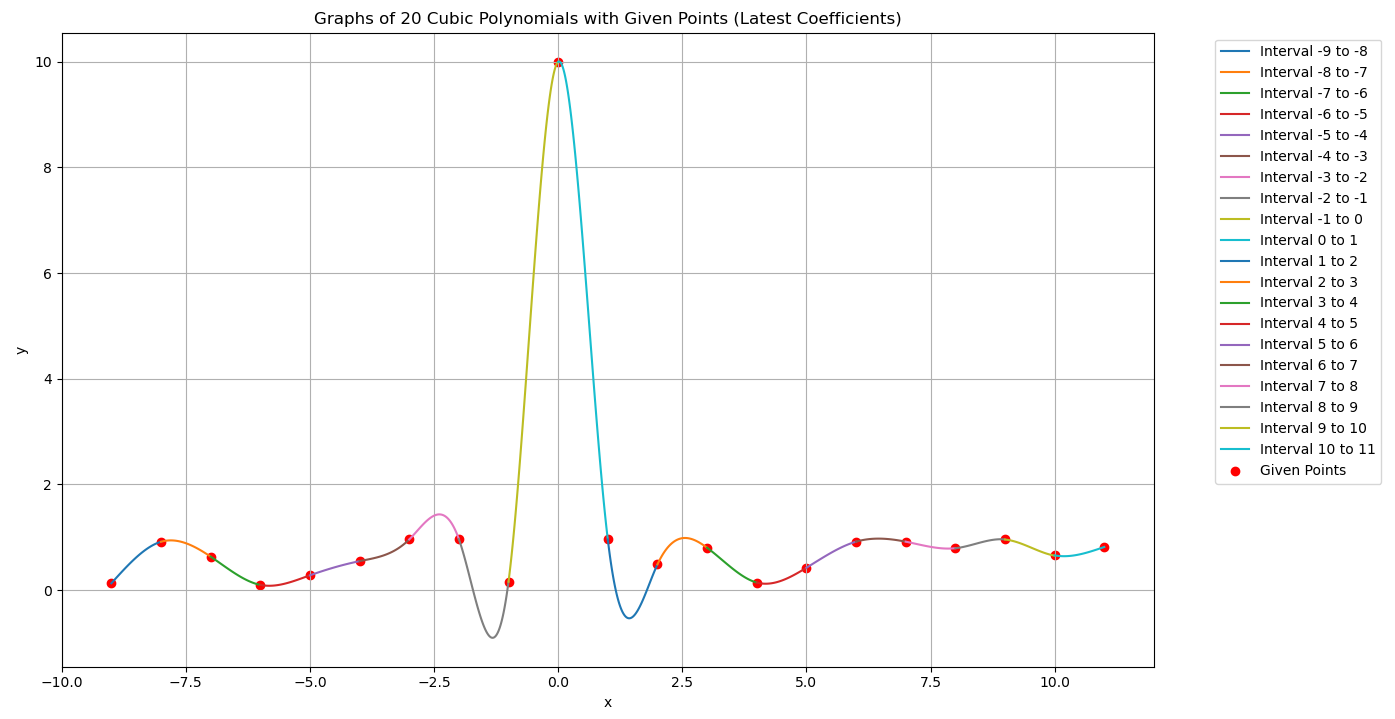
\includegraphics[scale=0.3]{Figure_2.png}
  \caption{更改后的结果可视化}
\end{figure}
\subsection{结果分析}
\begin{enumerate}
  \item 经计算验证,区间端点两侧一阶和二阶导数值近似相等.
  \item 通过观察可以发现,各个区间上的函数表达式均有改变,离被修改的点越远,改变越小.
\end{enumerate}


\bibliography{math}

\end{document}
\iffalse
\begin{figure}[h]
    \centering
    \includegraphics[scale=0.5]{name.png}
    \caption{name}
\end{figure}
\fi
